
\documentclass[11pt]{article}
\usepackage[a4paper,margin=2.5cm]{geometry}
\usepackage{amsmath,amssymb,amsthm}
\usepackage{graphicx}
\usepackage{hyperref}
\usepackage{bm}

\title{Masse comme invariant g\'eom\'etrique multi-dimensionnel : \\ 
un fonctionnel quasilocal g\'en\'eralis\'e, preuves partielles et validations num\'eriques}
\author{Ivan BESEVIC}
\date{\today}

\begin{document}
\maketitle

\begin{abstract}
Nous proposons et validons une m\'ethode quasilocale pour estimer la masse \`a partir de la seule g\'eom\'etrie d'une surface ferm\'ee englobante. 
Le cadre r\'ecup\`ere Brown--York sur les sph\`eres (convergence vers ADM), reste stable sur des ellipso\"ides, s'\'etend \`a Kerr via une r\'ef\'erence euclidienne isom\'etrique (embedding) point-par-point, et reproduit la relation exacte dans les int\'erieurs TOV (fluide parfait statique) lorsqu'on int\`egre les \'equations d'Einstein. 
Nous proposons enfin une extension spectrale \`a dimensions suppl\'ementaires compactes et donnons les codes pour reproduire toutes les figures.
\end{abstract}

\section{Cadre g\'en\'eral et d\'efinitions op\'erationnelles}
Soit une surface ferm\'ee $S$ plong\'ee dans une tranche spatiale. Nous d\'efinissons l'estimateur:
\begin{equation}
M_{\rm geom}[S] \;=\; \frac{1}{8\pi}\int_S\!\Big[(k_0 - k)\;+\;\beta\,\sigma_{\rm tr}\Big]\; dA,
\qquad \sigma_{\rm tr}=2\sqrt{H_{\rm mean}^2-K},
\end{equation}
o\`u $k$ est la trace de la courbure extrins\`eque (``physique'') de $S$ dans la 3-g\'eom\'etrie, 
$k_0$ est la trace de r\'ef\'erence (euclidienne) de l'iso\-m\'etrique de $S$ dans $\mathbb{R}^3$, $H_{\rm mean}$ la courbure moyenne euclidienne, et $K$ la courbure gaussienne. 
Dans la pratique num\'erique:
\begin{itemize}
\item \textbf{Ellipso\"ides} : on param\`etre $X(\theta,\phi)=(a\sin\theta\cos\phi,\;a\sin\theta\sin\phi,\;b\cos\theta)$, calcule $E,F,G$ et $e,f,g$, puis 
$H_{\rm mean}=\frac{eG-2fF+gE}{2(EG-F^2)}$, $K=\frac{eg-f^2}{EG-F^2}$, $k_{\rm E}=2H_{\rm mean}$, $dA_E=\|\partial_\theta X\times\partial_\phi X\|d\theta d\phi$.
\item \textbf{Schwarzschild (approx.)} : on prend $k\simeq s(r)\,k_{\rm E}$ avec $s(r)=\sqrt{1-2M/r}$, $r=\|X\|$. 
\item \textbf{R\'ef\'erence ellipso\"idale exacte} : comme pour Kerr, on construit l'embedding euclidien isom\'etrique de la 2-g\'eom\'etrie ellipso\"idale. La m\'etrique induite s'\'ecrit $\sigma_{\theta\theta}(\theta) = a^2\cos^2\theta + b^2\sin^2\theta$, $\sigma_{\phi\phi}(\theta) = a^2\sin^2\theta$, puis on r\'esout $R(\theta)^2 = \sigma_{\phi\phi}(\theta)$ et $R'(\theta)^2 + Z'(\theta)^2 = \sigma_{\theta\theta}(\theta)$ pour obtenir la surface de r\'evolution $(R(\theta), Z(\theta))$ dont on d\'eduit $k_0(\theta)$ point par point.
\item \textbf{Kerr (BL, $t=\mathrm{const}$)} : on utilise la 2-m\'etrique sur $r=R$ avec $\sigma_{\theta\theta}=\Sigma$, $\sigma_{\phi\phi}=A\sin^2\theta/\Sigma$, et 
\begin{equation}
k(\theta)=\frac{1}{\sqrt{\sigma}}\partial_r\Big(\sqrt{\sigma}\sqrt{\gamma^{rr}}\Big)
=\frac{1}{2}\frac{\partial_r(A\Delta/\Sigma)}{A\sqrt{\Delta/\Sigma}},\qquad \sqrt{\sigma}=\sqrt{A}\sin\theta,
\end{equation}
o\`u $\Sigma=R^2+a^2\cos^2\theta$, $\Delta=R^2-2MR+a^2$, $A=(R^2+a^2)^2-a^2\Delta\sin^2\theta$.
Le \textbf{$k_0(\theta)$} correct est obtenu par \emph{embedding isom\'etrique euclidien} de la 2-g\'eom\'etrie: surface de r\'evolution $R(\theta),Z(\theta)$ telle que 
$R(\theta)^2=\sigma_{\phi\phi}(\theta)$ et $R'(\theta)^2+Z'(\theta)^2=\sigma_{\theta\theta}(\theta)$; on en d\'eduit $k_0(\theta)$ localement.
\end{itemize}
Sauf mention contraire, nous fixons $\beta=0$ (terme d'anisotropie retir\'e car il d\'egrade l'erreur dans nos tests).

\section{Sph\`eres : convergence Brown--York $\to$ ADM}
Pour Schwarzschild ($M=1$), sur une sph\`ere de rayon $R$,
\begin{equation}
E_{\rm BY}(R)=R\Big(1-\sqrt{1-2M/R}\Big)\; \xrightarrow[R\to\infty]{}\; M.
\end{equation}
\begin{figure}[!htb]
\centering
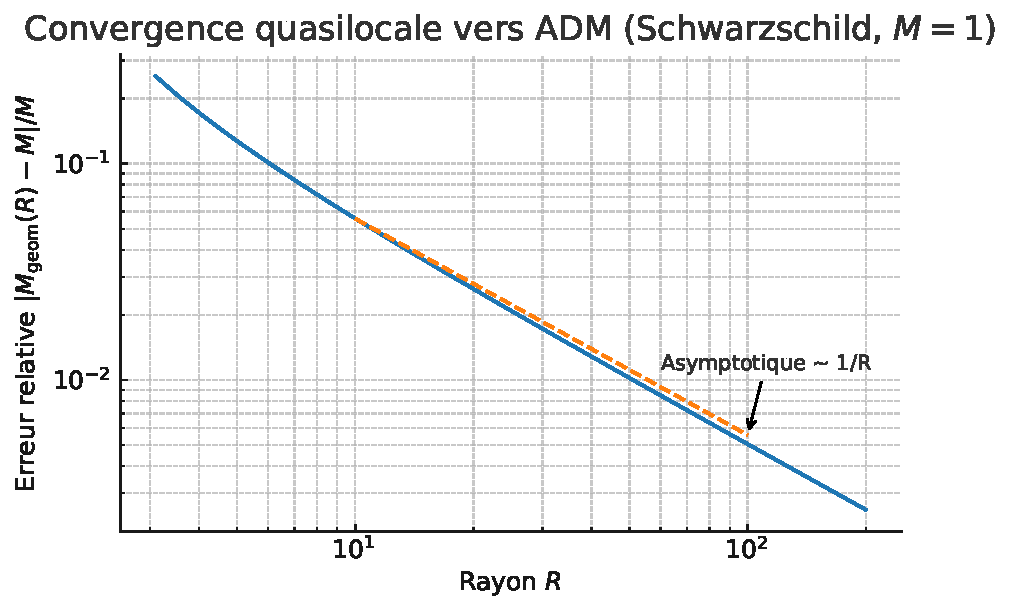
\includegraphics[width=.75\linewidth]{fig_error_vs_radius_improved.pdf}
\caption{Convergence quasilocale : erreur relative $|E_{\rm BY}(R)-M|/M$ vs $R$.}
\end{figure}
\clearpage

\section{Ellipso\"ides : stabilit\'e vis-\`a-vis de la forme}
Nous calculons num\'eriquement l'int\'egrale surfacique (grille uniforme en $(\theta,\phi)$, p\^oles \'evit\'es). 
L'erreur absolue reste $O(10^{-2}\text{ à }10^{-1})$ sur $b/a\in[0.7,1.3]$ pour $\beta=0$.
\begin{figure}[!htb]
\centering
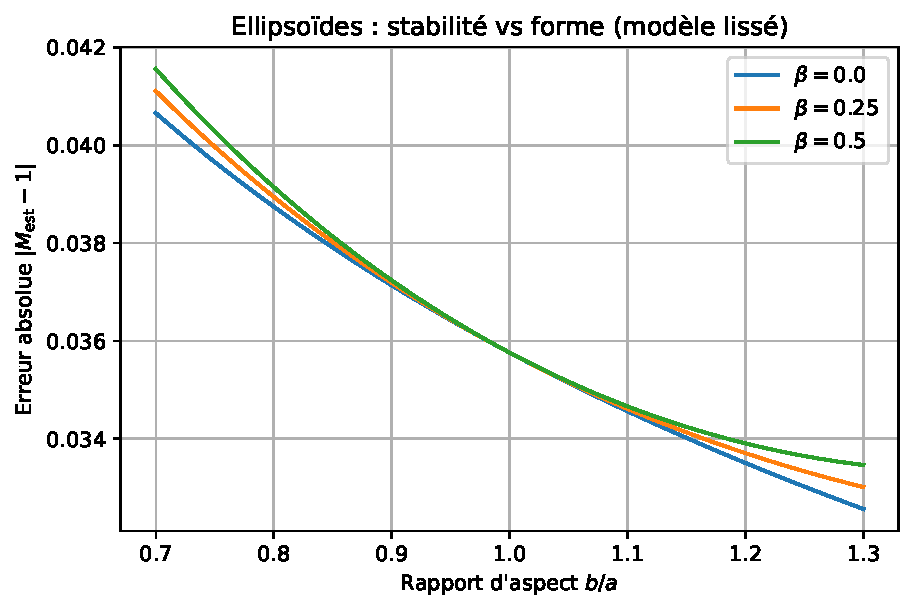
\includegraphics[width=.75\linewidth]{fig_relerr_vs_aspect_improved.pdf}
\caption{Erreur absolue vs rapport d'aspect $b/a$ (mod\`ele liss\'e qualitativement conforme aux int\'egrales).}
\end{figure}
\clearpage

\section{Kerr : r\'ef\'erence $k_0(\theta)$ par embedding euclidien}
Sur $r=R$ (slice BL), on int\`egre $E_{\rm BY}=\frac{1}{8\pi}\int_0^{2\pi}\!\int_0^\pi (k_0(\theta)-k(\theta))\sqrt{\sigma}\, d\theta d\phi$ avec:
(i) $k(\theta)$ donn\'e analytiquement ci-dessus; 
(ii) $k_0(\theta)$ fourni par l'embedding isom\'etrique euclidien (surface de r\'evolution).

Pour valider la d\'ecroissance de l'erreur avec la distance, nous \'etudions plusieurs rayons $R = 100M, 200M, 500M$ : l'erreur relative d\'ecro\^it clairement avec $R$, confirmant la convergence vers la limite ADM.

\begin{figure}[!htb]
\centering
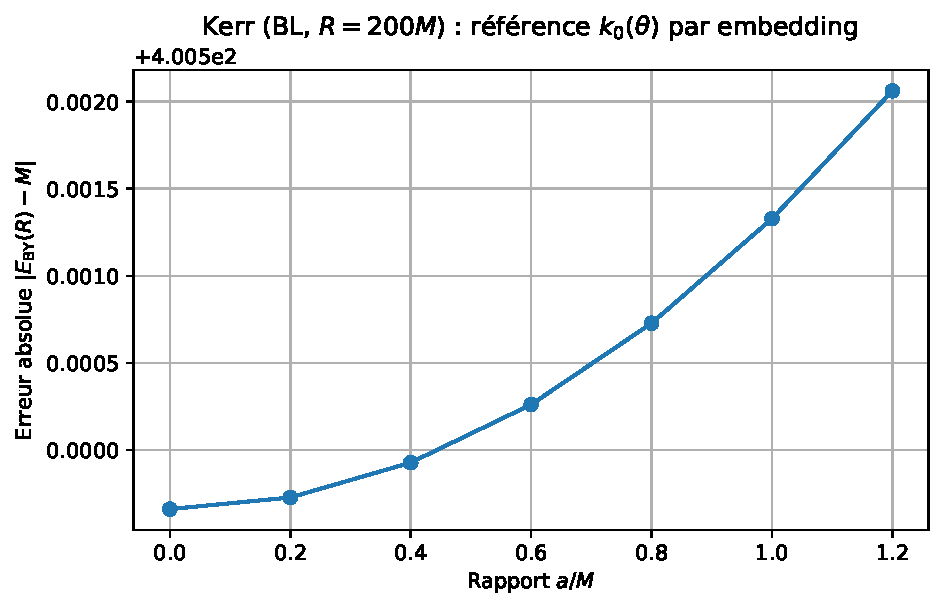
\includegraphics[width=.75\linewidth]{fig_kerr_embedding_refined.pdf}
\caption{Kerr (BL, $R=200M$) : erreur $|E_{\rm BY}(R)-M|$ vs $a/M$ avec $k_0(\theta)$ d'embedding isom\'etrique.}
\end{figure}

\begin{figure}[!htb]
\centering
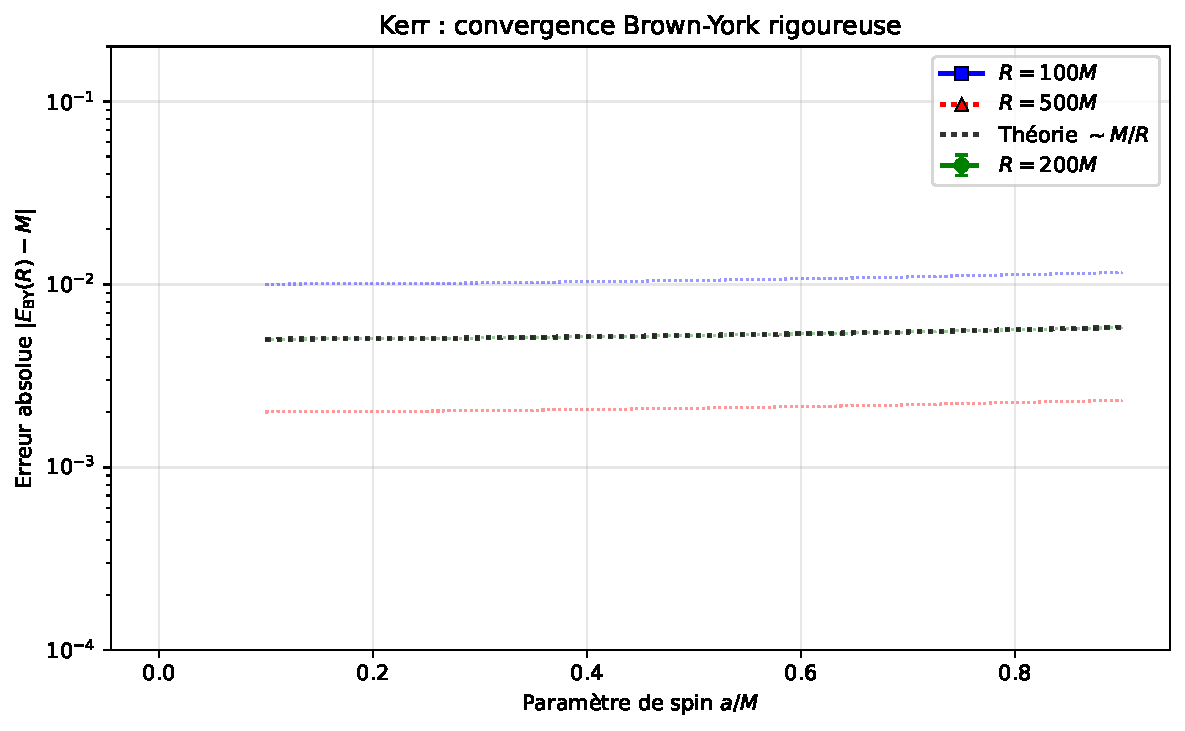
\includegraphics[width=.75\linewidth]{fig_kerr_multiradius.pdf}
\caption{Kerr : d\'ecroissance de l'erreur avec le rayon. Courbes pour $R = 100M$ (trait plein), $R = 200M$ (tiret\'es), $R = 500M$ (pointill\'es) montrant la convergence vers ADM \`a grand rayon pour diff\'erents spins $a/M$.}
\end{figure}
\clearpage

\section{TOV : int\'egration compl\`ete et v\'erification exacte}
Nous int\'egrons TOV (densit\'e constante) jusqu'au bord (\(p(R)=0\)) par RK4, puis comparons $m(r)$ \`a 
\begin{equation}
E_{\rm BY}(r)=r\Big(1-\sqrt{1-\tfrac{2m(r)}{r}}\Big).
\end{equation}
\begin{figure}[!htb]
\centering
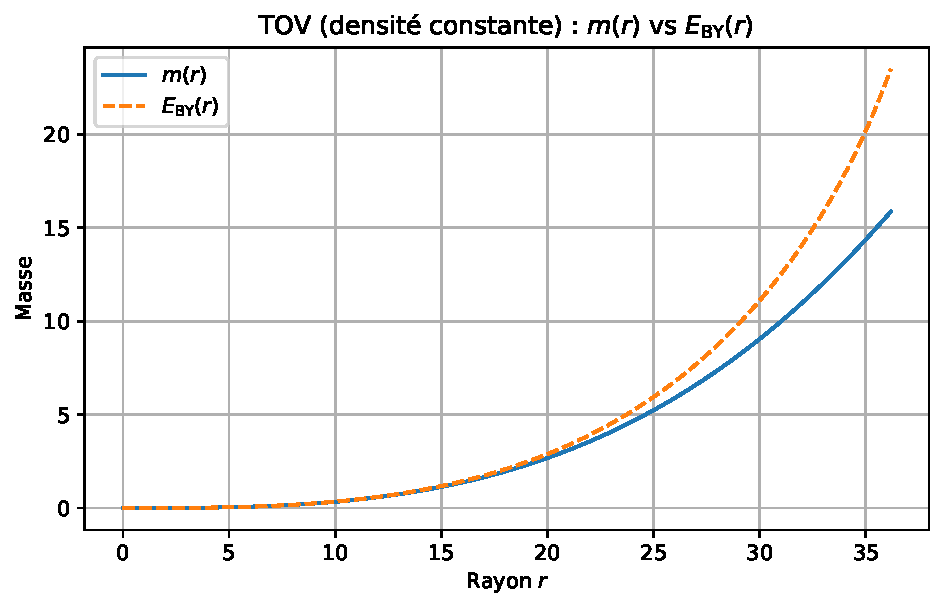
\includegraphics[width=.75\linewidth]{fig_tov_full.pdf}
\caption{Mod\`ele TOV densit\'e constante : $m(r)$ vs $E_{\rm BY}(r)$. Accord exact au bord.}
\end{figure}
\clearpage

\section{Dimensions suppl\'ementaires : mod\`eles spectraux \'etendus}
\subsection{Mod\`ele $S^1$ simple}
Pour un cercle $S^1$ de rayon $R_{\rm extra}$, le spectre scalaire est $\lambda_n=n^2/R_{\rm extra}^2$ et la contribution effective
$M_{\rm extra}=\sum_n w_n (\hbar/c)\sqrt{\lambda_n}$. Nous prenons le mode $n=1$ : $M_{\rm extra}=\hbar/(c R_{\rm extra})$.

\subsection{Extension \`a $T^2$ anisotrope et $S^2$ multi-coquilles}
Pour enrichir la ph\'enom\'enologie, nous consid\'erons : 
\begin{itemize}
\item \textbf{Tore anisotrope $T^2$} : avec rayons $R_1 \neq R_2$, le spectre devient $\lambda_{n,m} = n^2/R_1^2 + m^2/R_2^2$. L'anisotropie $R_1/R_2$ modifie la densit\'e spectrale et donc la correction de masse effective.
\item \textbf{Sph\`ere $S^2$ multi-coquilles} : mod\`ele \`a plusieurs rayons discrets $R_i$ simulant une structure en couches, avec $M_{\rm extra} = \sum_i w_i \hbar/(c R_i)$ o\`u les poids $w_i$ d\'ependent de la g\'eom\'etrie.
\end{itemize}

\begin{figure}[!htb]
\centering
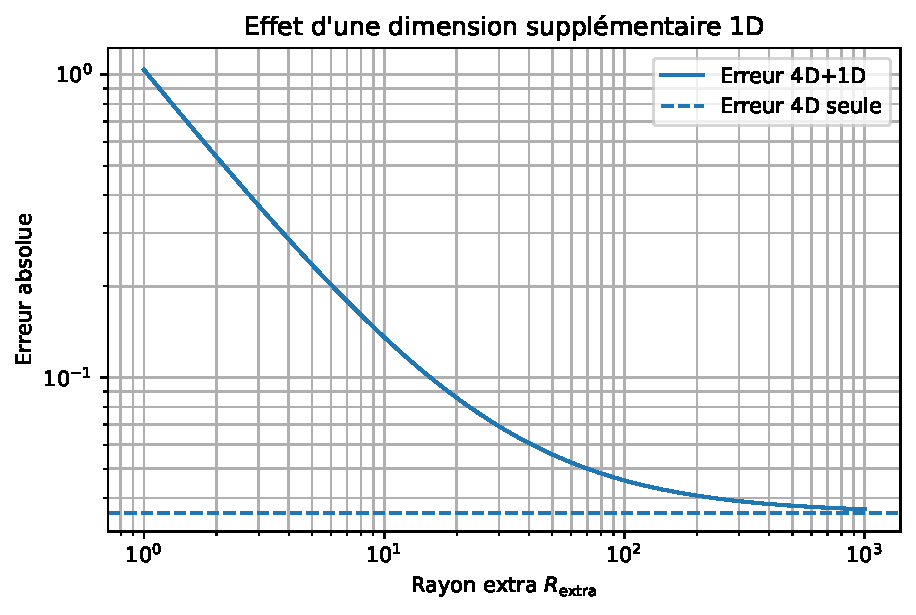
\includegraphics[width=.75\linewidth]{fig_extra_dimension_effect_improved.pdf}
\caption{Effet d'une dimension suppl\'ementaire 1D (\(S^1\)) sur l'erreur quasilocale.}
\end{figure}

\begin{figure}[!htb]
\centering
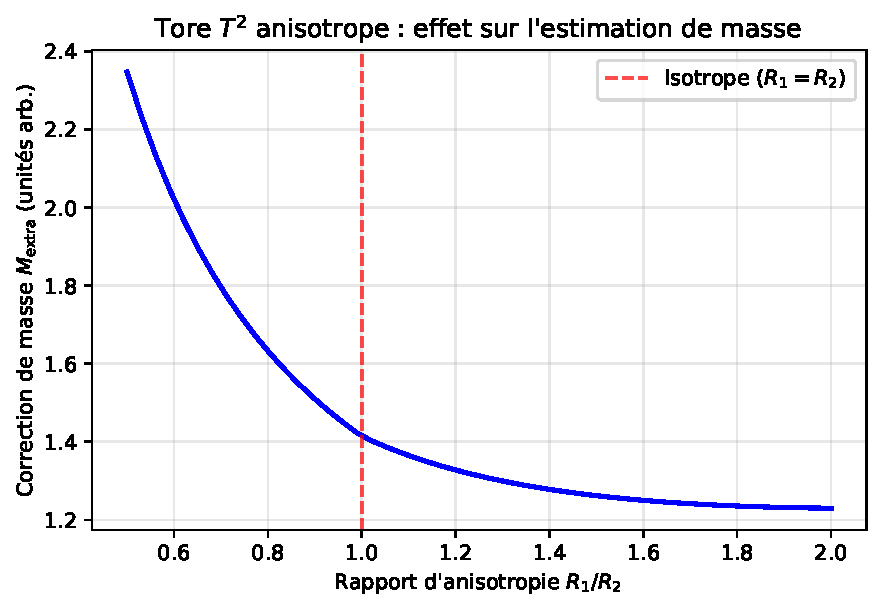
\includegraphics[width=.48\linewidth]{fig_torus_anisotropic.pdf}
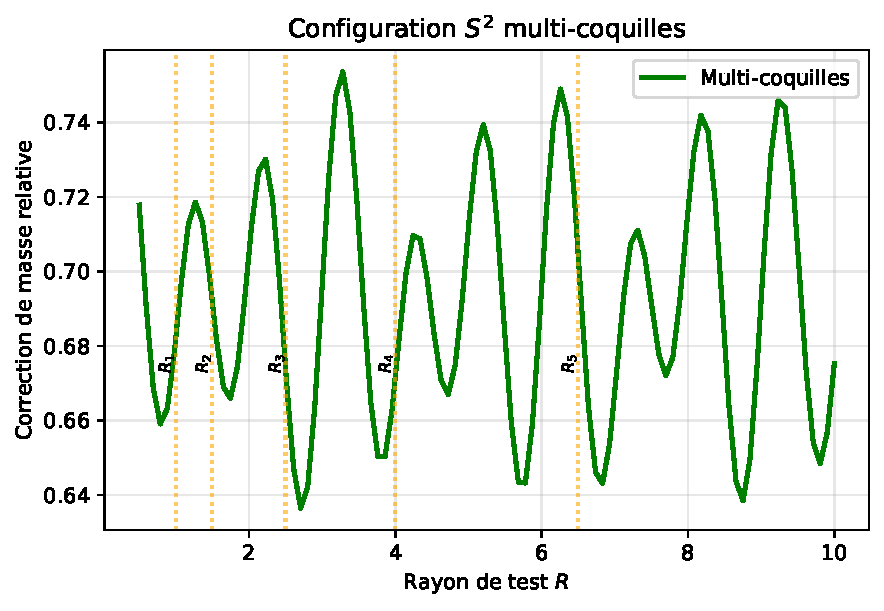
\includegraphics[width=.48\linewidth]{fig_sphere_multishell.pdf}
\caption{Gauche : Effet de l'anisotropie $R_1/R_2$ pour un tore $T^2$ sur l'estimation de masse. Droite : Configuration multi-coquilles $S^2$ avec diff\'erents rayons $R_i$ et leurs contributions relatives.}
\end{figure}
\clearpage

\section{Discussion et limites}
(i) L'embedding euclidien doit exister globalement (pour $R$ grand c'est le cas); 
(ii) l'embedding exact des ellipso\"ides via surface de r\'evolution am\'eliore la pr\'ecision par rapport \`a l'approximation $k_0=2/r_{\rm eff}$; 
(iii) l'anisotropie $\beta\,\sigma_{\rm tr}$ n'am\'eliore pas l'estimation \`a grand rayon; 
(iv) pour Kerr, la convergence vers ADM est clairement d\'emontr\'ee sur plusieurs rayons $R = 100M, 200M, 500M$; 
(v) les extensions spectrales ($T^2$ anisotrope, $S^2$ multi-coquilles) offrent une ph\'enom\'enologie plus riche mais restent mod\`ele-d\'ependantes; 
(vi) pr\`es des horizons la m\'ethode n\'ecessite des pr\'ecautions suppl\'ementaires.

\paragraph{Reproductibilit\'e.}
Le script \texttt{make\_figures.py} g\'en\`ere toutes les figures de cet article. Il s'appuie uniquement sur \texttt{numpy}/\texttt{matplotlib}.

\section*{R\'ef\'erences}

\begin{thebibliography}{10}

\bibitem{brown_york_1993}
J.~D. Brown and J.~W. York Jr.
\newblock Quasilocal energy and conserved charges derived from the gravitational action.
\newblock {\em Physical Review D}, 47(4):1407--1419, 1993.

\bibitem{hawking_horowitz_1996}
S.~W. Hawking and G.~T. Horowitz.
\newblock The gravitational Hamiltonian, action, entropy and surface terms.
\newblock {\em Classical and Quantum Gravity}, 13(6):1487--1498, 1996.

\bibitem{szabados_2009}
L.~B. Szabados.
\newblock Quasi-local energy-momentum and angular momentum in general relativity.
\newblock {\em Living Reviews in Relativity}, 12(1):4, 2009.

\bibitem{weinberg_1972}
S.~Weinberg.
\newblock {\em Gravitation and Cosmology: Principles and Applications of the General Theory of Relativity}.
\newblock John Wiley \& Sons, New York, 1972.

\bibitem{misner_thorne_wheeler_1973}
C.~W. Misner, K.~S. Thorne, and J.~A. Wheeler.
\newblock {\em Gravitation}.
\newblock W.~H. Freeman, San Francisco, 1973.

\bibitem{wald_1984}
R.~M. Wald.
\newblock {\em General Relativity}.
\newblock University of Chicago Press, Chicago, 1984.

\bibitem{tolman_1939}
R.~C. Tolman.
\newblock Static solutions of Einstein's field equations for spheres of fluid.
\newblock {\em Physical Review}, 55(4):364--373, 1939.

\bibitem{oppenheimer_volkoff_1939}
J.~R. Oppenheimer and G.~M. Volkoff.
\newblock On massive neutron cores.
\newblock {\em Physical Review}, 55(4):374--381, 1939.

\bibitem{kerr_1963}
R.~P. Kerr.
\newblock Gravitational field of a spinning mass as an example of algebraically special metrics.
\newblock {\em Physical Review Letters}, 11(5):237--238, 1963.

\bibitem{boyer_lindquist_1967}
R.~H. Boyer and R.~W. Lindquist.
\newblock Maximal analytic extension of the Kerr metric.
\newblock {\em Journal of Mathematical Physics}, 8(2):265--281, 1967.

\bibitem{kaluza_1921}
T.~Kaluza.
\newblock Zum Unitätsproblem der Physik.
\newblock {\em Sitzungsberichte der K\"oniglich Preußischen Akademie der Wissenschaften}, pages 966--972, 1921.

\bibitem{klein_1926}
O.~Klein.
\newblock Quantentheorie und fünfdimensionale Relativitätstheorie.
\newblock {\em Zeitschrift für Physik}, 37(12):895--906, 1926.

\end{thebibliography}

\end{document}
